\documentclass[acmsmall,nonacm,screen]{acmart}

\usepackage{mathpartir}
\usepackage{booktabs}
\usepackage{tikz}
\usetikzlibrary{automata,positioning}

\citestyle{acmauthoryear}
\settopmatter{printacmref=false}

\AtEndPreamble{\theoremstyle{acmdefinition}\newtheorem{remark}[theorem]{Remark}}

\newcommand{\kw}[1]{\mathsf{#1}}
\newcommand{\nm}[1]{\mathit{#1}}
\newcommand{\ask}[1]{\kw{ask}(#1)}
\newcommand{\propose}[1]{\kw{propose}(#1)}
\newcommand{\final}[1]{\kw{final}(#1)}
\newcommand{\edit}{\nm{edit}}
\newcommand{\test}{\nm{test}}
\newcommand{\commit}{\nm{commit}}
\newcommand{\push}{\nm{push}}

% A sentence that states a fact in words. The script has one check for every name.
\newcommand{\claim}[2]{#2}

% The rows of a table that the script writes.
\makeatletter
\newcommand{\rows}[1]{\@@input artifact/expected/#1.tex }
\makeatother

% written by learn.py; do not edit
\newcommand{\exAlphabetLearner}{286}
\newcommand{\exAlphabetSifted}{58}
\newcommand{\exAskedMean}{85}
\newcommand{\exAskedMeanClosing}{85}
\newcommand{\exAskedMeanPlain}{122}
\newcommand{\exBlocksAll}{508}
\newcommand{\exCellRows}{17}
\newcommand{\exCellWords}{43}
\newcommand{\exCellsAsked}{24}
\newcommand{\exCellsFree}{19}
\newcommand{\exChain}{100}
\newcommand{\exChainPaid}{100}
\newcommand{\exDialogueAsked}{25}
\newcommand{\exDialoguePlain}{34}
\newcommand{\exEven}{25}
\newcommand{\exExamples}{3,617}
\newcommand{\exExamplesClosing}{3,628}
\newcommand{\exExamplesPlain}{2,175}
\newcommand{\exGrowthLearner}{24}
\newcommand{\exGrowthList}{13,402}
\newcommand{\exGrowthPlain}{74}
\newcommand{\exLengthPlain}{5,615}
\newcommand{\exLengthSearch}{28}
\newcommand{\exLines}{900}
\newcommand{\exMutants}{six}
\newcommand{\exPaid}{22,687}
\newcommand{\exPolicies}{1,000}
\newcommand{\exRefusals}{29,231}
\newcommand{\exRefusedTasks}{1,000}
\newcommand{\exSeed}{2026}
\newcommand{\exShapeTasks}{300}
\newcommand{\exStatesAll}{6,887}
\newcommand{\exTasksEach}{150}


\begin{document}

\title{A Refusal Is a Counterexample: Learning What an Agent May Do}

\author{Claude-Fable-5.2}
\authornote{An AI model. The theorems about the learner are those of the theory of learning
with queries, carried over to a new setting; the proofs are on paper and have not been
checked by a machine. A script implements the protocol and tests the claims on random
policies. At the time of writing nobody has reviewed the paper.}

\begin{abstract}
A user who supervises an agent answers the same question many times: may I do this? Harnesses
offer a way out, the answer ``yes, and do not ask again'' for an action or a pattern of
commands. Such a rule has no memory of what happened before. It cannot say ``push only after
the tests have run'', and a user with a policy of that kind is asked forever. We read the
dialogue between agent and user as learning with queries. The policy of the user is a regular
language of allowed histories. A question about one sequence of actions is a membership
query. A plan that the agent proposes for approval is a subset query, and when the user
declines and says what is wrong, that is a counterexample; so is a task that the user allows
and that falls outside the approved plan. With the algorithm of Angluin the agent learns as
it works. We show that every plan it proposes is closed under beginnings, as a permission
must be; that it never acts outside what the user approved; and that, for a policy with $n$
states, the user declines a proposal or is consulted about allowed work at most $n$ times,
whatever the work is and however long. Work that the user refuses is different. We show
that an agent with these two kinds of question must ask about it again and again, whatever
it has learned, and that a third question removes this: is the plan all that I may do? With
it nothing is asked after the first task. Agents that ask before every action, that remember sequences, or that
keep lists of actions ask without end for a policy with memory. For a policy with four
states, ten thousand tasks cost an agent with lists \exGrowthList{} questions, and the
learner \exGrowthLearner{} questions and proposals together. A script tests the bounds on \exPolicies{} random policies and notices
\exMutants{} deliberate mistakes.
\end{abstract}

\keywords{automata learning, queries, permissions, human oversight, regular languages, agents}

\authorsaddresses{}

\maketitle

\section{Introduction}

An agent that acts in the world asks before it acts. May I run this command, edit this file,
push this branch? The user says yes or no. An earlier paper of this series treats one such
answer as a value that licenses one action~\cite{tpp4}, and another lets the agent ask for a
whole plan, a regular language of actions, in one question~\cite{tpp11}. Neither says which
plan to ask for. In practice the agent asks about single actions, and the user, tired of
answering, picks the option that harnesses provide for this: ``yes, and do not ask again''.
The harness adds a rule to a list, and the action, or every command that matches a pattern,
is allowed from then on~\cite{claudecodepermissions}. That people pay little attention to
what they are asked to permit is documented~\cite{felt2012}.

A list of allowed actions is a policy without memory. It says which actions are allowed, and
it cannot say when. But the policies that users have are often about when. Commit only what
was tested. Push only what was committed. Delete only what you created. Send at most three
messages. For such a policy the answer ``always'' is wrong for the very actions that matter,
a careful user never gives it, and the questions do not stop.

This paper takes the view that the agent is \emph{learning} the policy of the user, and
that the dialogue should be designed as a learner's dialogue. The policy is a set of
histories that the user allows. It is closed under beginnings, and we assume that it is
regular: the user distinguishes finitely many situations. The agent has three kinds of
question.
\begin{itemize}
\item \emph{May I do this?}, for a sequence of actions. In the theory of learning this is a
  membership query~\cite{angluin1988}.
\item \emph{May I work by this plan?}, for a plan, which is a regular language. The user
  approves the plan if everything in it is allowed, and otherwise points to something in it
  that is not. This is a subset query, and the reply to a declined plan is a counterexample.
\item \emph{Is this plan all that I may do?} The user confirms, or names something allowed
  that the plan leaves out. This is a superset query.
\end{itemize}
The first two have counterparts in today's harnesses: the question before an action, and the
approval of a plan. There is also a source of information that costs the user nothing: the
work itself. A task that the user allows and that the approved plan
does not cover shows that the plan is too small.

With these, the algorithm of \citet{angluin1987} for learning a regular language applies. It
needs an equivalence query, which no user could answer in one piece. Here its two halves are
answered apart, and the half that is hard for a person, to say what a plan leaves out, is
answered by the tasks as they come. The learner then needs only as many corrections as the
policy has states.

\paragraph{Results.} The plans that the learner proposes are closed under beginnings, so
they are permissions in the sense of the earlier paper (Lemma~\ref{lem:plans}). The agent
performs exactly the tasks that the policy allows, and only under an approved plan
(Theorem~\ref{thm:safe}). Over any sequence of tasks, the proposals that the user rejects
and the allowed tasks that fall outside the plan number at most $n$ together, for a policy
with $n$ states (Theorem~\ref{thm:no}), and the questions about sequences are bounded by a
polynomial in $n$, the number of actions, and the logarithm of the length of the longest
counterexample, plus one question for every refused task (Theorem~\ref{thm:asks}). That last term
cannot be avoided by any agent that only asks and proposes
(Proposition~\ref{prop:refusals}); with the third question it disappears, and all learning
happens during the first task (Theorem~\ref{thm:closing}). Against this stand three agents
that do not learn, or learn too little (Section~\ref{sec:others}). An agent that asks before
every action asks in proportion to its work. One that remembers the sequences it was allowed
asks once for every new sequence. One that keeps lists of actions asks, for every action
whose permission depends on the past, at every use.

Our main contributions are as follows:
\begin{itemize}
\item The reading of approval as learning with queries: asking is a membership query,
  proposing a plan is a subset query, a refusal is a counterexample, and the work supplies
  the other half of an equivalence query (Section~\ref{sec:model}).
\item A learning agent for which the bounds of the theory of learning hold in this setting,
  with plans that are closed under beginnings and with safety by construction
  (Section~\ref{sec:agent}).
\item The place of the closing question: without it, an agent that asks and proposes must
  keep asking about work that is refused, and with it nothing is asked after the first task
  (Section~\ref{sec:refused}).
\item Propositions that say what always asking, remembering sequences, and lists of actions
  cannot do, and what a proposal is worth compared with questions
  (Section~\ref{sec:others}).
\item Measurements on \exPolicies{} random policies and on policies of several shapes,
  including the costs that the bounds hide: long tasks and large sets of actions
  (Section~\ref{sec:eval}).
\end{itemize}
The theorems about the learner are Angluin's, and we claim no new mathematics for them. The
contribution is the correspondence, the two results about refused work and about lists,
and what all of it says about how agents should ask.

\section{Overview}
\label{sec:overview}

An agent works on a repository. Four actions matter here: $\edit$, $\test$, $\commit$, and
$\push$. The user has a policy and has never written it down: a commit needs a test since
the last edit, and a push needs a commit since the last edit. Figure~\ref{fig:plan} shows the
policy as an automaton with three states; a fourth, which refuses everything, is not drawn.
A history is allowed if the automaton can follow it.

\begin{figure}
\centering
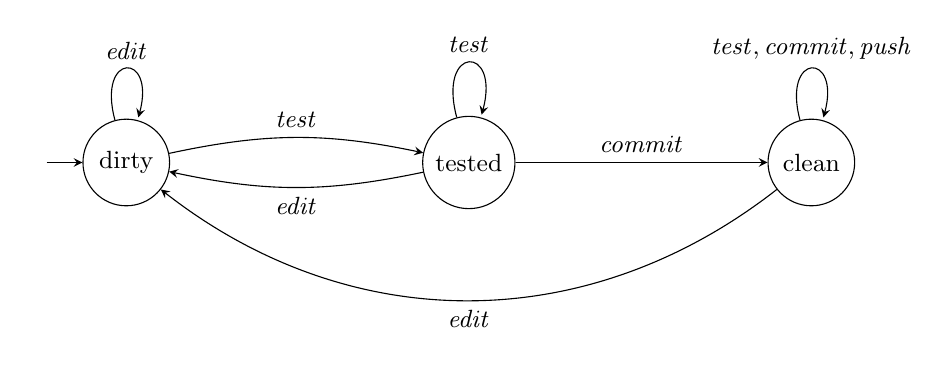
\begin{tikzpicture}[->, >=stealth, node distance=3.2cm, font=\small, every state/.style={minimum size=1.1cm}]
  \node[state, initial, initial text=] (d) {dirty};
  \node[state, right=of d] (t) {tested};
  \node[state, right=of t] (c) {clean};
  \path (d) edge[loop above] node {$\edit$} (d)
        (d) edge[bend left=12] node[above] {$\test$} (t)
        (t) edge[bend left=12] node[below] {$\edit$} (d)
        (t) edge[loop above] node {$\test$} (t)
        (t) edge node[above] {$\commit$} (c)
        (c) edge[loop above] node {$\test, \commit, \push$} (c)
        (c) edge[bend left=38] node[below] {$\edit$} (d);
\end{tikzpicture}
\caption{The policy of the example, and the plan that the learner proposes during the first
task. An action for which a state has no arrow is refused there.}
\Description{An automaton with three states, dirty, tested and clean. Edit leads to dirty
from every state. Test leads from dirty to tested and stays in tested and in clean. Commit
leads from tested to clean and stays in clean. Push is allowed in clean only.}
\label{fig:plan}
\end{figure}

\begin{table}
\caption{The dialogue for the first task, $\edit\ \test\ \commit\ \push$, in the order in
which the agent asks: first the left half, then the right.}
\label{tab:dialogue}
\small
\begin{tabular}{llll}
\toprule
the agent asks & answer & the agent asks & answer \\
\midrule
\rows{dialogue}
\bottomrule
\end{tabular}
\end{table}

\claim{example}{The first task is $\edit\ \test\ \commit\ \push$, and
Table~\ref{tab:dialogue} is the whole dialogue that the learning agent of
Section~\ref{sec:agent} has with the user about it: \exDialogueAsked{} questions and one
proposal, which is the policy and is approved.}

The agent begins with the four actions alone and learns that a commit and a push are refused
at the start. Its first guess is the simplest plan that fits: one state, in which edits and
tests are allowed and change nothing. The task is not in that plan, so the agent asks about
the task, and the user allows it. The guess is wrong, and the task shows it.

The agent now looks for the place where the guess goes wrong. In the guess an edit changes
nothing, so if the task is allowed, $\test\ \commit\ \push$ must be allowed without the edit.
The agent asks, and it is. In the guess a test changes nothing either, so $\commit\ \push$
would have to be allowed from the start, and it is not, because a commit is refused there. So
a test changes something that the guess does not track, and the ending $\commit\ \push$ shows
it: allowed after a test, refused before. The agent takes this ending as an
\emph{experiment}, a continuation that it tries after every history it tracks. The answers
split the one state of the guess in two, dirty and tested.

The second guess still refuses the task, since it has no state in which a push is allowed.
The same search finds that a commit changes something, and the experiment that shows it is
$\push$ alone. That gives the third state, clean. The third guess allows the task. The agent
proposes it; it is the policy of Figure~\ref{fig:plan}, and the user approves. From here on
the agent works without asking, however many tasks follow, as long as they are allowed.

The questions of Table~\ref{tab:dialogue} are many for one sitting. They are also all the
questions that allowed work will ever cost. An agent that asks before every action has
asked as many after a handful of tasks. An agent with a list of allowed actions asks once
about edits, once about tests, and then at every commit and every push, because for these
two the answer ``always'' would be false.

Now suppose that the agent sets out to do $\edit\ \commit$. The plan refuses it. But the
plan was built from the agent's own questions, and the user has approved only what is in it,
so the agent does not know that the user would refuse; it asks, and is told no. For
$\edit\ \edit\ \commit$ it has to ask again. Section~\ref{sec:refused} shows that no agent
can avoid this, unless the user answers one more question: \emph{is this plan all that I may
do?} After a yes the agent declines such tasks by itself.

Had the user's policy been stricter than the plan, say with at most three pushes, the user
would have declined the proposal and named a history with four pushes. The learner would
have taken that history as a counterexample of the other kind, searched it in the same way,
and proposed a larger automaton that counts.

\section{Policies, Questions, and Plans}
\label{sec:model}

Let $\Sigma$ be a finite set of actions. A \emph{history} is a word over $\Sigma$. The
\emph{policy} of the user is a language $U \subseteq \Sigma^{*}$ that is regular and closed
under beginnings: if the user allows a history, the user allows how it began. These are the
regular safety properties, the policies that a monitor can enforce by stopping an agent in
time~\cite{schneider2000}. We write $n$ for the number of states of the least complete
deterministic automaton for $U$; one of them refuses everything, unless $U$ is all of
$\Sigma^{*}$. A \emph{plan} is a regular language that is closed under beginnings, given as
a deterministic automaton in which a missing transition is a refusal; it is what the agent
may be allowed to work by, as in the earlier paper~\cite{tpp11}.

The user answers three questions.
\begin{itemize}
\item $\ask{w}$, for a history $w$: \emph{yes} if $w \in U$, and \emph{no} otherwise.
\item $\propose{H}$, for a plan $H$: \emph{approved} if $H \subseteq U$, and otherwise a
  history in $H \setminus U$.
\item $\final{H}$, for a plan $H$: \emph{confirmed} if $U \subseteq H$, and otherwise a
  history in $U \setminus H$.
\end{itemize}
We call them a question, a proposal, and a closing question, and we say that the agent
\emph{consults} the user when it puts any of them.

A \emph{task} is a history that the agent sets out to perform: the steps by which it means
to do what it was asked. The steps are the agent's choice, so a task may be allowed or
refused. Tasks arrive one after another, and each starts afresh: the policy speaks about the
history of one task. For each task the agent may consult the user, and then it performs the
task or declines it. An agent is \emph{safe} if it performs a task only when the user has
allowed it, by an answer or by the approval of a plan that contains the task, and
\emph{complete} if it declines only tasks that the policy refuses.

\begin{table}
\caption{The dialogue between agent and user, and the theory of learning with queries.}
\label{tab:dictionary}
\small
\begin{tabular}{ll}
\toprule
in the dialogue & in the theory \\
\midrule
the policy of the user & the language to be learned \\
the situations that the user distinguishes & the states of its least automaton \\
may I do this? & membership query \\
may I work by this plan? & subset query \\
is this plan all that I may do? & superset query \\
the history that the user names when declining & counterexample \\
an allowed task outside the approved plan & a counterexample that nobody had to look for \\
the answer ``always'' for an action & learning a language of the form $\Gamma^{*}$, $\Gamma \subseteq \Sigma$ \\
\bottomrule
\end{tabular}
\end{table}

The three questions are the membership, subset and superset queries of
\citet{angluin1988}; Table~\ref{tab:dictionary} sets the two vocabularies side by side. The
learner of \citet{angluin1987} uses membership queries and an \emph{equivalence query}: is
my hypothesis the language, and if not, give me a word on which they differ. A proposal and a
closing question are the two halves of that query, and they ask different things of the
user. To decline a proposal, the user has to find one thing in the plan that is not wanted,
which is what reviewing a plan means. To decline a closing question, the user has to think of
something wanted that the plan leaves out. For work that is allowed, the second half need
not be asked. A plan that allows too little shows itself when an allowed task falls outside
it, and until then it does no harm.

\begin{definition}[Counterexample]
\label{def:cex}
For a plan $H$, a \emph{counterexample} is a history on which $H$ and the policy differ. It
reaches the agent in one of three ways: as the history that the user returns to
$\propose{H}$, which is in $H \setminus U$; as the history that the user returns to
$\final{H}$, which is in $U \setminus H$; or as a task outside $H$ that the user allows when
asked, which is in $U \setminus H$ as well.
\end{definition}

\section{The Learning Agent}
\label{sec:agent}

\subsection{The Table}

The learner keeps an observation table in the manner of \citet{angluin1987}: a list $S$ of
\emph{access words}, closed under beginnings and starting with the empty word; a list $E$ of
\emph{experiments}, also starting with the empty word; and the user's answer for every
history $s\,e$ and $s\,a\,e$ with $s \in S$, $a \in \Sigma$, $e \in E$. The \emph{row} of a
history $w$ maps each experiment $e$ to the answer for $w\,e$. Two histories with different
rows are continued by different sets of allowed histories, so they lead the least automaton
of the policy to different states~\cite{nerode1958}: there are at most $n$ different rows.
The access words have pairwise different rows. The table is \emph{closed} if the row of every
$s\,a$ is the row of some access word, and the learner closes it by adding $s\,a$ to $S$
whenever its row is new.

From a closed table the learner builds its \emph{hypothesis}: an automaton with one state for
the row of every allowed access word, the row of the empty word as its start, and a
transition by $a$ from the row of $s$ to the row of $s\,a$ when $s\,a$ is allowed. The empty
word is an experiment and the policy is closed under beginnings, so a refused history has
the row that says no everywhere. At most one access word is refused. It stands for the
refusing state and is not a state of the hypothesis.

\begin{lemma}[Hypotheses are plans]
\label{lem:plans}
Every hypothesis of the learner is closed under beginnings.
\end{lemma}

\begin{proof}
The automaton has transitions only between rows of allowed histories, and a missing
transition is a refusal. So a history that it follows has only beginnings that it follows.
\end{proof}

\paragraph{Answers that need no question.} Much of the table fills itself. If a beginning of
$w$ was refused, $w$ is refused. If $w$ was allowed, or continued to an allowed history,
$w$ is allowed. What the plan that the user approved last allows is allowed. A history that
the user named when declining a proposal is refused, and one named in reply to a closing
question is allowed. The learner asks only when none of these applies.

\begin{figure}
\centering
\small
\begin{tabular}{lccc}
\toprule
history & $\varepsilon$ & c p & p \\
\midrule
\rows{cells}
\bottomrule
\end{tabular}
\caption{The table of the learner at the end of the dialogue of Table~\ref{tab:dialogue}.
Actions are abbreviated by their first letters. Above the line are the access words, below
it their successors; the columns are the experiments. An answer in parentheses was not asked
for: it follows from another answer.}
\Description{A table with seventeen rows of histories and three columns of experiments.
Four rows are access words: the empty word, commit, test, and test commit. Many of the
answers are in parentheses.}
\label{fig:cells}
\end{figure}

Figure~\ref{fig:cells} shows the table at the end of the dialogue of
Section~\ref{sec:overview}. It has \exCellRows{} rows and three experiments, and its cells
hold \exCellWords{} different histories, of which the agent asked about \exCellsAsked{}; the
other \exCellsFree{} follow from closure under beginnings. \claim{cells}{The one question of
Table~\ref{tab:dialogue} that is not a cell of the table is the question about the task
itself.} The second access word, $\commit$, is the refused one.

\subsection{Counterexamples}

Let $w = a_1 \cdots a_k$ be a counterexample for the hypothesis $H$. For $0 \le i \le k$,
let $H$ follow $a_1 \cdots a_i$ to the state with access word $s_i$, and let $\alpha_i$ be
the answer for $s_i\, a_{i+1} \cdots a_k$; if $H$ refuses $a_1 \cdots a_i$, let $\alpha_i$ be
\emph{no}. Then $\alpha_0$ is the user's answer for $w$, since $s_0$ is the empty word, and
$\alpha_k$ is the answer of $H$, since the access word of a state is allowed. The two
differ. So $\alpha_{i-1} \neq \alpha_i$ for some $i$, and a binary search finds such an $i$
with at most $\lceil \log_2 k \rceil$ questions~\cite{rivest1993}. The learner adds the
ending $a_{i+1} \cdots a_k$ to its experiments and closes the table. We call this a
\emph{correction}. Section~\ref{sec:overview} went through two of them.

\begin{lemma}[A correction adds an access word]
\label{lem:progress}
After a correction the table has one access word more, at least.
\end{lemma}

\begin{proof}
Let $i$ be the place that the search found, and $e = a_{i+1} \cdots a_k$. If $H$ refused
$a_1 \cdots a_{i-1}$, both $\alpha_{i-1}$ and $\alpha_i$ would be \emph{no}. So $H$ follows
$a_1 \cdots a_{i-1}$ to the state of $s_{i-1}$. If $H$ had no transition by $a_i$ there,
$s_{i-1}\,a_i$ would be refused, and with it $s_{i-1}\,a_i\,e$, so again both answers would
be \emph{no}. So the transition exists, which means that $s_{i-1}\,a_i$ had the row of
$s_i$. The answers for $s_{i-1}\,a_i\,e$ and $s_i\,e$ are $\alpha_{i-1}$ and $\alpha_i$, and
they differ. With $e$ among the experiments, the row of $s_{i-1}\,a_i$ is no longer the row
of $s_i$. It is not the row of another access word either, since it differed from those
before and a new experiment does not make rows equal. So the table is not closed, and
closing it adds an access word.
\end{proof}

The learner keeps every counterexample that it has received. After a correction the new
hypothesis may still be wrong about one of them. Then the learner corrects again, with the
same counterexample, before it consults the user about anything else: it shows nobody a plan
that disagrees with a counterexample it knows.

A simpler learner adds \emph{every} ending of $w$ to the experiments~\cite{maler1995}. It
needs no search, the ending that the search would find is among those it adds, so
Lemma~\ref{lem:progress} holds for it, and its next hypothesis is right about $w$ at
once~\cite{angluin1987}. It asks more questions, \exDialoguePlain{} for the task of
Section~\ref{sec:overview} where the search needs \exDialogueAsked{}, and, as
Section~\ref{sec:eval} shows, it needs fewer counterexamples. We call it the \emph{plain}
learner.

\subsection{Learning While Working}
\label{sec:working}

The agent keeps the plan that the user approved last; at the start there is none. For a task
$t$ it proceeds as follows.
\begin{enumerate}
\item If $t$ is in the approved plan, perform $t$.
\item Otherwise, if the hypothesis refuses $t$, ask about $t$, unless the answer is known. If
  the user allows $t$, it is a counterexample: correct the table and repeat this step.
\item If the hypothesis is not the approved plan, propose it. If the user returns a history,
  it is a counterexample: correct the table and go back to step~2. If the user approves, the
  hypothesis is the approved plan from now on.
\item Perform $t$ if the approved plan contains it, and decline it otherwise.
\end{enumerate}
After every task the approved plan is the hypothesis of the table. A task that is outside
the approved plan when it arrives is the only occasion on which the user is consulted.

\begin{theorem}[Safe and complete]
\label{thm:safe}
The learning agent is safe and complete, and every plan that it works by is a subset of the
policy.
\end{theorem}

\begin{proof}
It performs a task only in steps 1 and 4, under an approved plan that contains the task, and
the user approves a plan only if it is within $U$. For completeness, let $t$ be allowed and
outside the plan. Step~2 repeats until the hypothesis allows $t$, and every repetition is a
correction, of which there are finitely many by Lemma~\ref{lem:progress}. Step~3 returns to
step~2 whenever it changes the table, so when it ends, the hypothesis is approved and
allows~$t$.
\end{proof}

\begin{theorem}[Allowed work interrupts the user at most $n$ times]
\label{thm:no}
Let the policy have $n$ states. Over every sequence of tasks, of any length, the learner
receives at most $n - 1$ counterexamples. Hence the proposals that the user rejects and the
allowed tasks that arrive outside the approved plan are at most $n$ together.
\end{theorem}

\begin{proof}
When a counterexample is received, the hypothesis is wrong about it, so at least one
correction follows. Every correction adds an access word (Lemma~\ref{lem:progress}). There
are at most $n$ access words, because their rows differ, and the table starts with one. A
rejected proposal yields a counterexample. So does an allowed task that arrives outside the
approved plan, since the plan is the hypothesis; the exception is the first task, which
arrives when there is no plan and may be allowed by the first hypothesis.
\end{proof}

\begin{theorem}[Questions]
\label{thm:asks}
Let $m$ be the length of the longest counterexample and $r$ the number of refused tasks that
the agent asks about. Over every sequence of tasks, the learning agent puts at most
$n^2\,(1 + |\Sigma|) + (n - 1)\,\lceil \log_2 m \rceil + n + r$ questions. With the plain
learner the bound is $n\,(1 + |\Sigma|)\,(1 + m\,(n - 1)) + r$.
\end{theorem}

\begin{proof}
There are at most $n$ access words, each with $|\Sigma|$ successors, and at most $n$
experiments: the empty word and one for each of at most $n - 1$ corrections. That bounds
the cells of the table. Each correction searches with at most $\lceil \log_2 m \rceil$
questions. Each task that arrives outside the plan costs at most one question about itself;
at most $n$ of these tasks are allowed, by Theorem~\ref{thm:no}. The learner asks about no
other histories, and about none twice. The plain learner does not search, has at most
$1 + m\,(n - 1)$ experiments, and an allowed task that it asks about is a cell of its
table.
\end{proof}

\begin{corollary}[In the limit]
\label{cor:limit}
After finitely many tasks the agent consults the user about refused tasks only. If every
history of the policy is the beginning of a later task again and again, the approved plan
becomes the policy.
\end{corollary}

\begin{proof}
By Theorems~\ref{thm:no} and~\ref{thm:asks} the other questions and the proposals are
bounded. As long as the plan is smaller than the policy, some later task is allowed and
falls outside it.
\end{proof}

The bound of Theorem~\ref{thm:no} is in the spirit of the mistake bounds of
\citet{littlestone1988}: the number of times that the learner is wrong does not depend on
how long it works.

\subsection{Tasks That the User Refuses}
\label{sec:refused}

A refused task outside the plan costs a question in step~2, and nothing is learned from the
answer, because the hypothesis was right. The term $r$ of Theorem~\ref{thm:asks} can grow
with the work. This is not a weakness of the learner.

\begin{proposition}[Without a closing question, refusals cost]
\label{prop:refusals}
Let an agent be safe and complete, and let it consult the user by questions and proposals
only. Let $t$ be a refused task such that no beginning of $t$, and not $t$ itself, is among
the histories that the user has refused so far, in reply to a question or to a proposal.
Then the agent consults the user at least once more before it declines $t$.
\end{proposition}

\begin{proof}
Let $U'$ be $U$ together with $t$ and its beginnings. It is regular and closed under
beginnings. Every answer that the user has given so far is a right answer for the policy $U'$
as well. An answer \emph{yes} stays right because $U \subseteq U'$, and so does an approval.
An answer \emph{no} was given for a history that $U$ refuses and that is not a beginning of
$t$, so $U'$ refuses it. A history that the user returned to a proposal $H$ is in $H$ and,
for the same reason, outside $U'$. So nothing that the agent has seen tells $U$ from $U'$.
Under $U$ the task must be declined, because the agent is safe, and under $U'$ it must be
performed, because the agent is complete.
\end{proof}

One reply refuses one history. In the policy of Section~\ref{sec:overview} the histories
$\edit^k\ \commit$, for $k \ge 1$, are all refused, none is a beginning of another, and
their proper beginnings are allowed. So a hundred tasks of this kind cost a hundred
consultations, even for an agent whose plan is already the policy. What such an agent
lacks is not knowledge of the policy but the user's word that there is nothing more.

That word is the reply to the closing question. The agent \emph{with the closing question}
changes step~3: after an approval it puts $\final{H}$. A history that the user returns is a
counterexample; the agent corrects the table and goes back to step~2. Once the user
confirms, the plan is \emph{closed}, and from then on the agent declines every task outside
it without asking.

\begin{theorem}[With the closing question]
\label{thm:closing}
The agent with the closing question is safe and complete. It consults the user during its
first task only. It receives at most $n - 1$ counterexamples and puts at most
$n^2\,(1 + |\Sigma|) + (n - 1)\,\lceil \log_2 m \rceil + 1$ questions, and from the second
task on its plan is the policy.
\end{theorem}

\begin{proof}
The first task ends when a plan $H$ has been approved and closed, so $H \subseteq U
\subseteq H$. Performing the tasks in the plan and declining all others is then safe and
complete, and needs nobody. A history returned to a closing question is a counterexample to
the hypothesis, so Lemma~\ref{lem:progress} bounds the counterexamples as in
Theorem~\ref{thm:no}. The questions are those of Theorem~\ref{thm:asks}, except that only
the first task can cost a question about itself.
\end{proof}

With proposals and closing questions the user is the teacher that Angluin's algorithm
assumes, and Theorem~\ref{thm:closing} is her theorem. The agent of
Section~\ref{sec:working} is the same learner with half a teacher. It learns only as much of the policy as the work needs, and it pays for
that with a question for every task that the user refuses.

\section{Agents That Do Not Learn}
\label{sec:others}

We compare with three agents. All are safe and complete.

\emph{Always asking.} The agent asks before every action of every task, and stops a task at
the first refusal, which we count as declining it; the same holds for the next two.

\emph{Remembering sequences.} The agent asks before an action unless the same history with
the same action was answered before.

\emph{Lists.} The agent keeps a list of actions that are always allowed and a list of
actions that are never allowed, and asks before an action that is on neither. The user may
answer ``yes, always'' or ``no, never'', which puts the action on a list. We assume a careful
user, who gives such an answer only when it is true: \emph{always} when the policy allows
the action after every allowed history, \emph{never} when it refuses it after every allowed
history.

\begin{proposition}[Asking, and remembering]
\label{prop:ask}
For allowed tasks, always asking costs as many questions as the tasks have actions, and
remembering sequences costs one question for every distinct nonempty beginning of a task.
For the policy that allows everything, which has one state, this is up to $|\Sigma| +
|\Sigma|^2 + \cdots + |\Sigma|^k$ questions for tasks of length $k$, where the learning
agent asks $|\Sigma|$ questions and makes one proposal.
\end{proposition}

\begin{proof}
The first two counts are the definitions. For the policy that allows everything, the learner
asks about the $|\Sigma|$ single actions, finds one row, and proposes the plan that allows
everything, which is approved.
\end{proof}

\begin{proposition}[What lists cannot learn]
\label{prop:list}
Let $a$ be an action that the policy allows after some allowed history and refuses after
another. Then the agent with lists asks whenever a task comes to $a$, in every sequence of
tasks. If there is no such action, it asks at most $|\Sigma|$ questions in all.
\end{proposition}

\begin{proof}
For such an action both ``always'' and ``never'' are false. The careful user gives neither,
so the action is on no list. For every other action, the first question is answered
``always'' or ``never''.
\end{proof}

The proposition draws the line exactly. A policy is within the reach of lists when it is a
set of actions, the language $\Gamma^{*}$ for some $\Gamma \subseteq \Sigma$. Every policy
with memory, which is every policy whose least automaton has two states, other than the
refusing one, that allow different actions, has an action that is asked about at every use.

The learner depends on its proposals. An agent that may only ask about sequences can still
identify a policy, in principle, and for some policies it cannot do so with few questions.

\begin{proposition}[Asking is not enough]
\label{prop:block}
For a word $b$ of $k \ge 2$ letters over two letters, let $U_b$ be the policy that allows
every history in which $b$ does not occur as a block. It has $k + 1$ states. An agent that
identifies the policy among all $U_b$ by questions about histories of at most $\ell$ letters
needs at least $(2^k - 1) / (\ell - k + 1)$ questions in the worst case. The learning agent
has one proposal rejected, and its second proposal is the policy.
\end{proposition}

\begin{proof}
A history of $\ell$ letters contains at most $\ell - k + 1$ blocks of $k$ letters. An
adversary answers \emph{yes} as long as some block occurs in none of the histories asked
about, and may still choose any such block as $b$. Each question removes at most $\ell - k +
1$ candidates, and one candidate must remain alone. The learning agent finds both letters
allowed and first proposes the plan that allows everything. The user returns a history $w$
that contains $b$, and the learner corrects its table until its hypothesis refuses $w$. Such
a hypothesis has an access word $s$ and a letter $a$ for which $s\,a$ is refused, so $b$ is
an ending of $s\,a$ and $s$ has at least $k - 1$ letters. The access words are closed under
beginnings, so $k$ of them are allowed, and with the refused one the table has $k + 1$
different rows, one for every state of the least automaton of $U_b$. The hypothesis is then
that automaton.
\end{proof}

This is the pattern of the lower bounds for learning with membership queries
alone~\cite{angluin1981}. In our setting it says what a review of a plan is worth: the user
who looks at a plan and says ``not this'' gives in one answer what exponentially many yes
and no answers would be needed for. Table~\ref{tab:buys} collects what each kind of answer
buys.

\begin{table}
\caption{What each kind of answer buys, for a policy with $n$ states. Each line assumes the
answers of the lines above it.}
\label{tab:buys}
\small
\begin{tabular}{lll}
\toprule
the user answers & what allowed work costs & what refused tasks cost \\
\midrule
questions about histories & grows with the work (Prop.~\ref{prop:ask}) & grows as well \\
``always'' and ``never'' & bounded only without memory (Prop.~\ref{prop:list}) & the same \\
proposals of plans & at most $n$ interruptions (Thm.~\ref{thm:no}) & one question each (Prop.~\ref{prop:refusals}) \\
the closing question & the same, all in the first task & nothing (Thm.~\ref{thm:closing}) \\
\bottomrule
\end{tabular}
\end{table}

\section{Evaluation}
\label{sec:eval}

The artifact is one Python script of about \exLines{} lines with no dependencies. It
implements policies as automata, a user who answers the three questions and counts them, the
learner with and without the search, the learning agent with and without the closing
question, and the three other agents. The command \texttt{make -C artifact check} runs the
script and compares its output with the files from which this paper takes its numbers and
the rows of its tables. Tables~\ref{tab:growth}, \ref{tab:refused} and~\ref{tab:alphabet}
give one number for an agent: its consultations, which are questions, proposals and closing
questions together.

\paragraph{The bounds.} The script draws \exPolicies{} random policies over four actions with
two to ten states, from a generator with seed \exSeed{}, and for each a sequence of
\exTasksEach{} random tasks of up to twelve actions, about a fifth of which the policy
refuses, \exRefusals{} in all. It runs four agents on each: with the search or plain, and
with or without the closing question. \claim{bounds}{For every policy and each of the four
agents, the agent performs exactly the tasks that the policy allows, every approved plan is
within the policy by a search that is written apart from the user's, the counterexamples are
at most the number of states less one, and the questions are within the bounds of
Theorems~\ref{thm:asks} and~\ref{thm:closing}.} The policies have \exStatesAll{} states in
all. Without the closing question, the agent with the search receives \exExamples{}
counterexamples and the plain one \exExamplesPlain{}; not counting the questions about
refused tasks, they ask \exAskedMean{} and \exAskedMeanPlain{} questions for a policy on
average. So the search saves questions and costs corrections: an agent that asks less knows
less when it proposes. \claim{exact}{With this many tasks the last plan is the policy itself
for every one of the policies, also without the closing question.}

\paragraph{The closing question.} \claim{closing}{With the closing question, every final
plan is the policy, and no agent consults the user after its first task.} The agent with the
search then receives \exExamplesClosing{} counterexamples and asks \exAskedMeanClosing{}
questions for a policy on average. \claim{refusals-cost}{Without the closing question the
same agent puts \exPaid{} questions about refused tasks. For each of them the script builds
the policy of Proposition~\ref{prop:refusals}, which allows the task as well, and checks that
every answer that the user had given until then is a right answer for that policy too.}

\begin{table}
\caption{Five policies, each with \exShapeTasks{} random allowed tasks: the questions of the
three agents that do not learn, and for the learner its questions, its proposals, the
proposals that were rejected, and the tasks that arrived outside the approved plan.}
\label{tab:shapes}
\small
\setlength{\tabcolsep}{4pt}
\begin{tabular}{lrrrrrrrr}
\toprule
 & & \multicolumn{3}{c}{questions without learning} & \multicolumn{4}{c}{the learner} \\
policy & states & always & remembered & lists & questions & proposals & rejected & outside \\
\midrule
\rows{shapes}
\bottomrule
\end{tabular}
\end{table}

\paragraph{Shapes.} Table~\ref{tab:shapes} compares the agents on five policies: everything
is allowed; everything but pushes; the policy of Section~\ref{sec:overview}; at most three
pushes; and one release, which is edits and tests, then one commit, then one push, and
nothing more. \claim{shapes}{For the two policies without memory the lists need at most
one question for every action, and the learner one question for every action and one
proposal. For the three with memory the learner consults the user less than a ninth as often
as the lists do, and in every line the rejected proposals and the tasks outside the plan
together are at most the number of states. Proposals are rejected only for the two policies
that count, the three pushes and the one release; for the first, the learner proposes a plan
with pushes without limit, and the user names the history with four.}

\begin{table}
\caption{The policy of Section~\ref{sec:overview} with growing numbers of allowed tasks: the
consultations of each agent.}
\label{tab:growth}
\small
\begin{tabular}{rrrrrr}
\toprule
tasks & always & remembered & lists & plain learner & learner \\
\midrule
\rows{growth}
\bottomrule
\end{tabular}
\end{table}

\paragraph{Growth.} \claim{growth}{Table~\ref{tab:growth} repeats the comparison for the
policy of Section~\ref{sec:overview} with up to ten thousand tasks. The consultations of the
learner do not grow, and those of the lists do, because only edits and tests can be allowed
for good. The lists have asked more than the learner ever asks after \exEven{} tasks, and by
then the learner has finished.} The plain learner needs \exGrowthPlain{} consultations where
the learner with the search needs \exGrowthLearner{}.

\begin{table}
\caption{The policy of Section~\ref{sec:overview} with \exRefusedTasks{} tasks, a growing
number of which the policy refuses: the consultations of each agent.}
\label{tab:refused}
\small
\begin{tabular}{rrrrrr}
\toprule
refused tasks & always & remembered & lists & learner & learner with closing \\
\midrule
\rows{refused}
\bottomrule
\end{tabular}
\end{table}

\paragraph{Refused tasks.} \claim{refused}{Table~\ref{tab:refused} mixes refused tasks into
the work. The learner without the closing question pays for them, as
Proposition~\ref{prop:refusals} says it must, and the learner with it does not: its
consultations stay below forty in every line. For the \exChain{} tasks $\edit^k\ \commit$
after the task of Section~\ref{sec:overview}, the learner without it puts \exChainPaid{}
questions and the learner with it none.} Even where half of the tasks are refused, the learner without the closing
question consults the user far less often than the lists do: allowed work costs it nothing,
and some refusals follow from earlier ones, since a task that begins with a refused history
is refused.

\begin{table}
\caption{The policy of Section~\ref{sec:overview} with two hundred allowed tasks of a given
length: the questions of the plain learner and of the learner with the search.}
\label{tab:lengths}
\small
\begin{tabular}{rrr}
\toprule
actions in a task & plain learner & learner \\
\midrule
\rows{lengths}
\bottomrule
\end{tabular}
\end{table}

\paragraph{Long tasks.} A counterexample is as long as the task that it comes from.
\claim{lengths}{Table~\ref{tab:lengths} shows what that costs the plain learner, which makes
every ending of a counterexample an experiment: \exLengthPlain{} questions for tasks of eight
hundred actions. The learner with the search asks \exLengthSearch{}, hardly more than for
short tasks.} This is the factor $m$ of Theorem~\ref{thm:asks} against its logarithm.

\begin{table}
\caption{The policy of Section~\ref{sec:overview} over more actions, all but four of which
are allowed everywhere and change nothing: the consultations of the lists, of the learner,
and of a learner that first asks of every action whether it ever matters.}
\label{tab:alphabet}
\small
\begin{tabular}{rrrr}
\toprule
actions & lists & learner & learner told what matters \\
\midrule
\rows{alphabet}
\bottomrule
\end{tabular}
\end{table}

\paragraph{Many actions.} The bound of Theorem~\ref{thm:asks} is linear in the number of
actions, and an agent has many. Table~\ref{tab:alphabet} takes three hundred tasks for the
policy of Section~\ref{sec:overview} and puts further actions in between, such as reading a
file, which the policy allows everywhere and which change nothing. \claim{alphabet}{The lists pay one question for
each new action. The learner pays one for each new action in each state and for each
experiment, \exAlphabetLearner{} consultations for thirty-two actions. A learner that may
first ask of every action whether it ever matters, and that leaves out the actions for which
the answer is no, pays one question for each again: \exAlphabetSifted{} consultations.} The
answer ``it never matters'' says more than ``always'': the action is allowed everywhere, and
the same histories are allowed with it and without. With that answer the learner can drop
the action from every history before it asks.

\begin{table}
\caption{The policies of Proposition~\ref{prop:block} for blocks of $k$ letters: what the
learner needs to learn the policy exactly, and the number of blocks among which an agent
without proposals has to find the forbidden one.}
\label{tab:blocks}
\small
\begin{tabular}{rrrrrr}
\toprule
$k$ & states & questions & proposals & rejected & blocks \\
\midrule
\rows{blocks}
\bottomrule
\end{tabular}
\end{table}

\paragraph{Blocks.} \claim{blocks}{Table~\ref{tab:blocks} shows the learner on the policies of
Proposition~\ref{prop:block}: a number of questions that grows with $k$ and not with $2^k$.
For every one of the \exBlocksAll{} blocks of two to eight letters, both learners have one
proposal rejected, and their second proposal is the policy.}

\paragraph{Deliberate mistakes.} The script plants \exMutants{} mistakes and runs its tests
against each: a user who approves every plan; a learner that records a refusal as a
permission; a learner that ignores counterexamples; a learner that forgets that the
beginnings of an allowed history are allowed; an agent that acts on its hypothesis before
the user has approved it; and an agent that declines whatever is outside its plan without
asking. \claim{all-noticed}{Each is noticed: the learner that forgets by a count of questions
that goes up, and the others by a check that fails.} The checks are those of the paragraph
on the bounds, together with two that the script makes of the learner itself: that every
correction adds an access word, and that the dialogue about a task comes to an end.

\paragraph{What the tests do not show.} The user of the script is a program that knows its
policy as an automaton and answers every question correctly and at once. It returns a
shortest counterexample, which a person may not. The cost that matters in practice is the
attention of a person, and a question about a sequence of twelve actions is not one click.
The counts say how the numbers of consultations compare; they do not say what a consultation
costs.

\section{Discussion}
\label{sec:discussion}

\paragraph{What the user is asked to do.} The protocol moves work from many small answers to
few large ones. A proposal is an automaton, and to review it the user must find, if there is
one, a history that it allows and that the user does not want. For small plans that is a
matter of reading: the plan of Figure~\ref{fig:plan} has three states. The harness can help.
It can show a new plan as a change to the plan that was approved before. It can show, for
every transition of the plan, a shortest history that uses it. And the user who approves too quickly is not lost: when an action
happens that the user did not want, the user's objection is a counterexample that arrives
late. The plan is withdrawn, the answers that the learner took from it are asked for again,
the learner is corrected, and Theorem~\ref{thm:no} still counts the corrections, though the
action has happened.

\paragraph{What the closing question asks.} To confirm that a plan is all, the user has to
be sure that nothing else is wanted. That is a judgment about the future, and a user may
prefer not to make it. Nothing forces it: without the closing question the agent is still
safe, complete, and bounded in what allowed work costs. A user who confirms too early gets
an agent that declines too much, and will notice, because a declined task is reported. The
user's reply that the task is allowed is a counterexample that reopens the plan. So the
answer ``that is all'' is a statement about the plan of today, and Theorem~\ref{thm:no}
counts the reopenings.

\paragraph{Questions about sequences.} The learner asks about histories that nobody
intends to perform, such as $\edit\ \commit\ \push$ in Table~\ref{tab:dialogue}. Users
answer such questions when they explain a policy to a colleague, and a harness can take
many of the answers from what it has seen: a history that the user allowed in the past is
allowed, and so is every beginning of it. Other learners ask
less~\cite{isberner2014,vaandrager2022}, and they keep a bound of the same kind on
counterexamples, which is the number that this paper is about. The comparison of our two learners shows the
exchange that they all face: fewer questions leave more for the user to correct.

\paragraph{Policies that change.} A user may change the policy. A stricter policy shows
itself as an objection to an action under an approved plan, a looser one as a task that the
user allows and the plan refuses. Both are counterexamples, and the learner can be restarted
with the old answers that are still true. The bounds then hold between two changes.

\paragraph{Approvals as values.} An approved plan is a permission of the kind that the
earlier papers of this series track in types: a token for a regular language that is used up
action by action~\cite{tpp11}. Nothing changes there. What this paper adds is where the plan
comes from. It also meets the paper on obligations~\cite{tpp12} at one point: the least
request that a harness computes when an agent may not finish is a question of the first
kind, and the answers to such requests are data for the learner.

\section{Related Work}
\label{sec:related}

\paragraph{Learning with queries.} \citet{gold1967} asked what can be learned from examples
in the limit. \citet{angluin1987} showed that a regular language is learned in polynomial
time from membership queries and equivalence queries with counterexamples, and
\citet{angluin1988} set out the kinds of queries, among them the subset and superset queries
that we use for the approval and the closing of a plan. Without equivalence queries the
number of membership queries is exponential in the worst case~\cite{angluin1981}.
\citet{maler1995} add the endings of a counterexample as experiments, which is our plain
learner; the binary search is due to \citet{rivest1993}; \citet{kearns1994} present the
algorithm with a tree in place of the table, and \citet{isberner2014} and
\citet{vaandrager2022} reduce the membership queries further. The bound on corrections is a
mistake bound in the sense of \citet{littlestone1988}. Our theorems about the learner are
these results in a setting where the two halves of the equivalence query are answered by a
person and by the stream of tasks.

\paragraph{Learning automata in programming languages.} Specifications of how a library is
meant to be called have been mined from the traces of programs that use
it~\cite{ammons2002} and learned with Angluin's algorithm from the library
itself~\cite{alur2005}. The same algorithm finds the assumption under which a component is
correct~\cite{cobleigh2003} and builds models of protocols and devices from
tests~\cite{vaandrager2017}. In all of these the teacher is a program, and the equivalence
query is replaced by a model checker or by a test suite that is complete up to a bound on
the states~\cite{chow1978}. Here the teacher is the user of an agent, the language is what
the user permits, and the count that matters is how often the user must object. Synthesis
guided by counterexamples~\cite{solarlezama2006} and by an oracle~\cite{jha2010} has the same
loop of candidate and counterexample; there the candidate is a program, and the answers come
from a verifier or from an oracle for inputs and outputs.

\paragraph{People as teachers.} A person has been the source of answers before. A wizard
for privacy settings asks its user about a few cases and infers the rest of the user's
preferences~\cite{fang2010}; a synthesizer of temporal specifications interacts with its user
to choose among candidates~\cite{gavran2020}; and a language model has answered the
membership queries of Angluin's algorithm about a task that is described in
words~\cite{vazquezchanlatte2024}. In the last of these the model is the teacher. Here it is
the learner, the person is the teacher, and what is learned is a permission, so that a wrong
generalization must be caught before the agent acts on it. That is the role of the
proposal.

\paragraph{Policies over histories.} Our policies are the safety properties that security
automata enforce~\cite{schneider2000}, monitors that can also change the sequence of actions
enforce more~\cite{ligatti2005}, and a policy over the actions on one object is a
typestate~\cite{strom1986}. That work starts from a policy that someone has written down.
This paper is about the policy that nobody has written down, and about getting it from its
owner with few questions.

\paragraph{Permissions for agents.} Harnesses ask before actions and keep lists of what is
allowed~\cite{claudecodepermissions}, and what requests for permission achieve with the
people who answer them has been measured~\cite{felt2012}. The earlier papers of this series
give approvals types~\cite{tpp4}, say when an action needs approval because of what the
agent has read~\cite{tpp7}, and make plans regular languages that are approved as a
whole~\cite{tpp11}. None of them says how a plan comes to be proposed. The practice of
binding numbers and marked sentences to the script follows~\cite{tpp10}.

\section{Limits and Conclusion}
\label{sec:limits}

\paragraph{Limits.} The policy is regular and over a finite set of actions. Real actions
have arguments, and a policy such as ``delete only the files that you created'' needs one
state for every file; automata over data can be learned~\cite{cassel2016}, and we have not
tried. A history is the history of one task, so a policy that counts over a day is outside
the model unless the day is one task. The user answers correctly and consistently. The user
reviews plans, which is harder than answering about one action, and we have counted reviews
and not measured them. The questions about sequences are many for one sitting, they grow
with the number of actions, and our remedy for that is one more kind of answer. And the plan
that the learner proposes is the smallest automaton that fits what it knows, which may allow
much that was never discussed; that is the nature of generalizing, and it is the reason why
the user's review is part of the protocol and cannot be skipped.

\paragraph{Conclusion.} A user who answers an agent is teaching it, and the questions of
today's harnesses are those of a poor student: the same ones again, and a notebook that
cannot record a condition. With the two kinds of question that agents already have, and
Angluin's learner, the user objects at most as often as the policy has states. A third
question settles what the agent may not do. The plan is not a convenience on top of
permissions. It is the form in which a policy with memory can be asked for at all.

\bibliographystyle{ACM-Reference-Format}
\bibliography{refs}

\end{document}
